\documentclass{article}
\usepackage{graphicx}
\usepackage[margin=1.5cm]{geometry}
\usepackage{amsmath}

\begin{document}

\title{Introduction to Vectors: Displacement and Velocity}
\author{Prof. Jordan C. Hanson}

\maketitle

\begin{abstract}
The purpose of this group activity is to practice problem-solving with vectors.  \textit{Displacement} is a vector that represents translational motion.  This is distinct from \textit{distance}, which is a scalar quantity representing the total amount of length an object has traversed.  \textit{Velocity} is displacement divided by time duration.  In this activity, we will attempt to navigate a submarine such that it is not eliminated by either a torpedo or an undersea wall of rock.
\end{abstract}

\section{The Problem Statement - The Hunt for Red October}

\textit{The Red October} is the name of a Russian nuclear submarine (from the novel by Tom Clancy, 1984), captained by Cpt. Marco Rameus.  Red October is being pursued by a torpedo in a large undersea canyon.  The torpedo has a higher speed than the submarine.  Both are traveling in a straight line initially, meaning at some time the torpedo will hit the submarine.

Let a two-dimensional \textit{x-y} coordinate system describe the area.  The appropriate unit of distance for the area is the kilometer, or 1000.0 m.  The initial position of the submarine is $\vec{x}_{i,s} = (-1.0, 0.0)$ km.  The initial position of the torpedo is $\vec{x}_{i,t} = (-2.0, 0.0)$ km.  The initial velocity of the submarine is $\vec{v}_{i,s} = (v_x,0.0)$ km/h.  The initial velocity of the torpedo is $\vec{v}_{i,t} = (50.0,0.0)$ km/h.  The situation is depicted in Fig. \ref{fig:hunt1}.

\begin{figure}[hb]
\centering
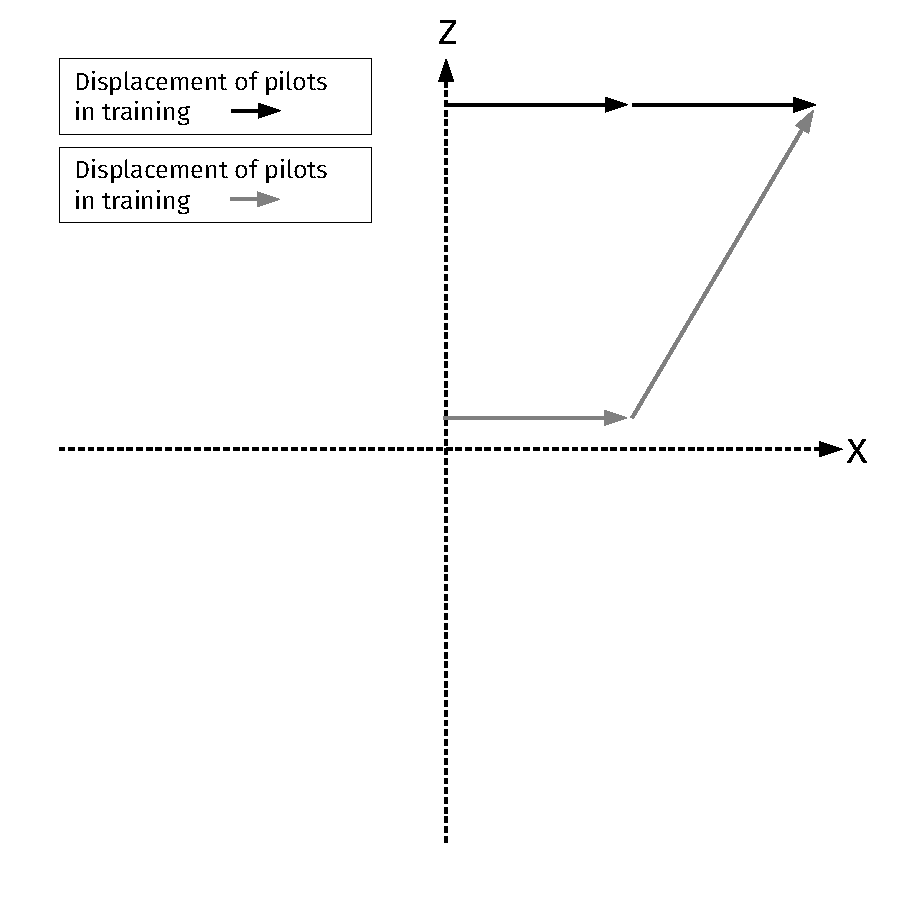
\includegraphics[width=0.3\textwidth]{TheHuntForRedOctober1.pdf}
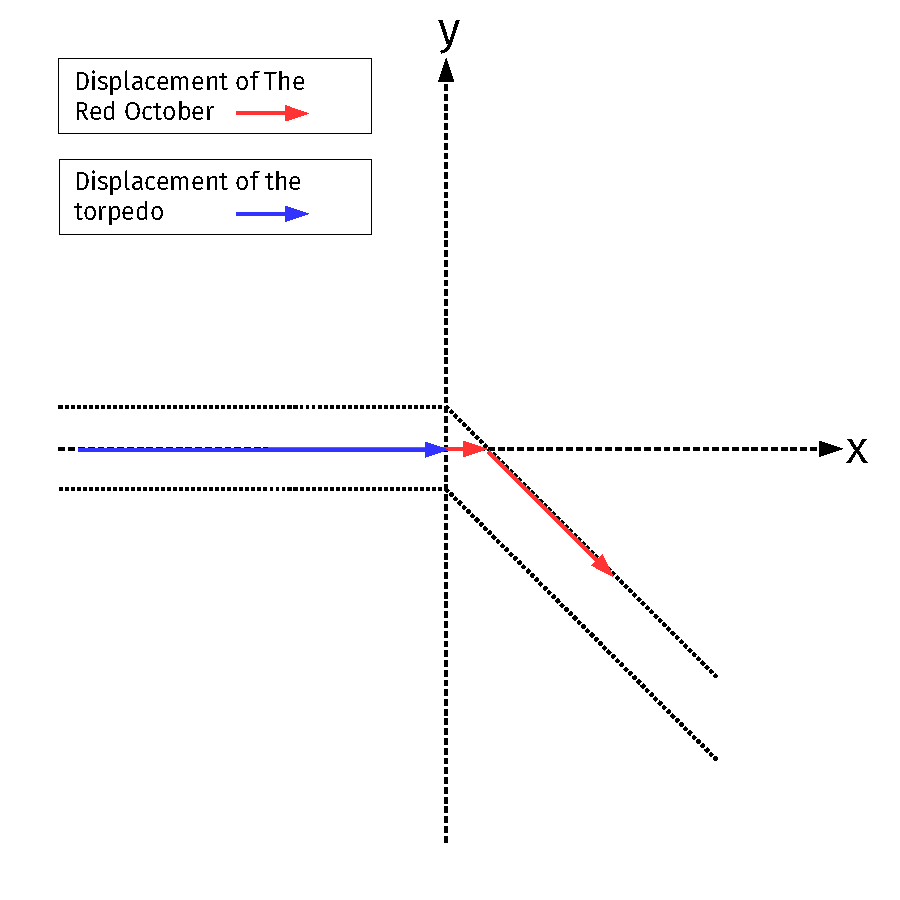
\includegraphics[width=0.3\textwidth]{TheHuntForRedOctober2.pdf}
\caption{\label{fig:hunt1}  (Left) The submarine prepares for a right turn at an angle of 45 degrees.  The lane (fine-dashed lines) is 1.0 km wide, or 0.5 km on either side of the submarine. (Right) The submarine captain sails up to the canyon wall, then turns South (downward in the diagram) at an angle of -45.0 degrees.}
\end{figure}

\section{Initial Displacements}

\textit{Displacement} is formally defined as the difference between the final position and the initial position:

\begin{equation}
\Delta \vec{x} = \vec{x}_f - \vec{x}_i
\end{equation}

What is the displacement of the submarine from the initial position $\vec{x}_{i,s}$ as it reaches the canyon wall?  What is the displacement of the torpedo as it reaches the canyon wall? \\ \vspace{1cm}

$\Delta \vec{x}_s = (?,?) ~~~~~~~~~~~~~~~~~~~~ \Delta \vec{x}_t = (?,?)$

\section{Initial Velocities}

Average \textit{velocity} is formally defined as the ratio between displacement and some time duration $\Delta t = t_f - t_i$.

\begin{equation}
\vec{v} = \frac{\Delta \vec{x}}{\Delta t}
\end{equation}

Multiplying both sides by $\Delta t$ yields

\begin{equation}
\vec{v}\Delta t = \Delta \vec{x} \label{eq:Eq1}
\end{equation}

Taking the \textbf{absolute value} or \textbf{magnitude} of a vector is the same as using the Pythagorean theorem to determine the length of the vector.  Taking the magnitude of both sides of Eq. \ref{eq:Eq1} is written like

\begin{align}
|\vec{v}\Delta t| &= |\Delta \vec{x}| \\
v\Delta t &= \Delta x \label{eq:Eq2}
\end{align}

Assume the situation begins with $t_i = 0$.  Using Eq. \ref{eq:Eq2}, determine when the torpedo hits the canyon wall, if the velocity remains constant. \\ \vspace{1cm}

$t_f = ?$ \\

What speed ($v_x$) must Captain Rameus choose, if he is to turn at the moment the torpedo hits the canyon wall? \\ \vspace{3cm}

$v_x = ?$ \\

Note that he \textbf{deliberately chooses a lower speed} to allow the torpedo to reach the wall at the same time as the submarine!

\section{Final Displacement and Average Velocity}

Captain Rameus continues at the same speed, but the boat turns at an angle of -45 degrees with respect to the x-axis.  After 3 minutes, what is the final location of the submarine? \\ \vspace{2cm}

$\vec{x}_{f,s} = (?,?)$ \\

What is the final \textit{displacement} of the submarine?  What is the average velocity of the submarine ? \\ \vspace{2cm}

$\Delta \vec{x}_s = \vec{x}_{f,s} - \vec{x}_{i,s} = (?,?) ~~~~~~~~~~~~~~~~~~~~ \vec{v}_s = \frac{\Delta \vec{x}_s}{\Delta t} = (?,?)$ \\

\end{document}
